\section{Method}


\begin{figure}[t]
	\centering
	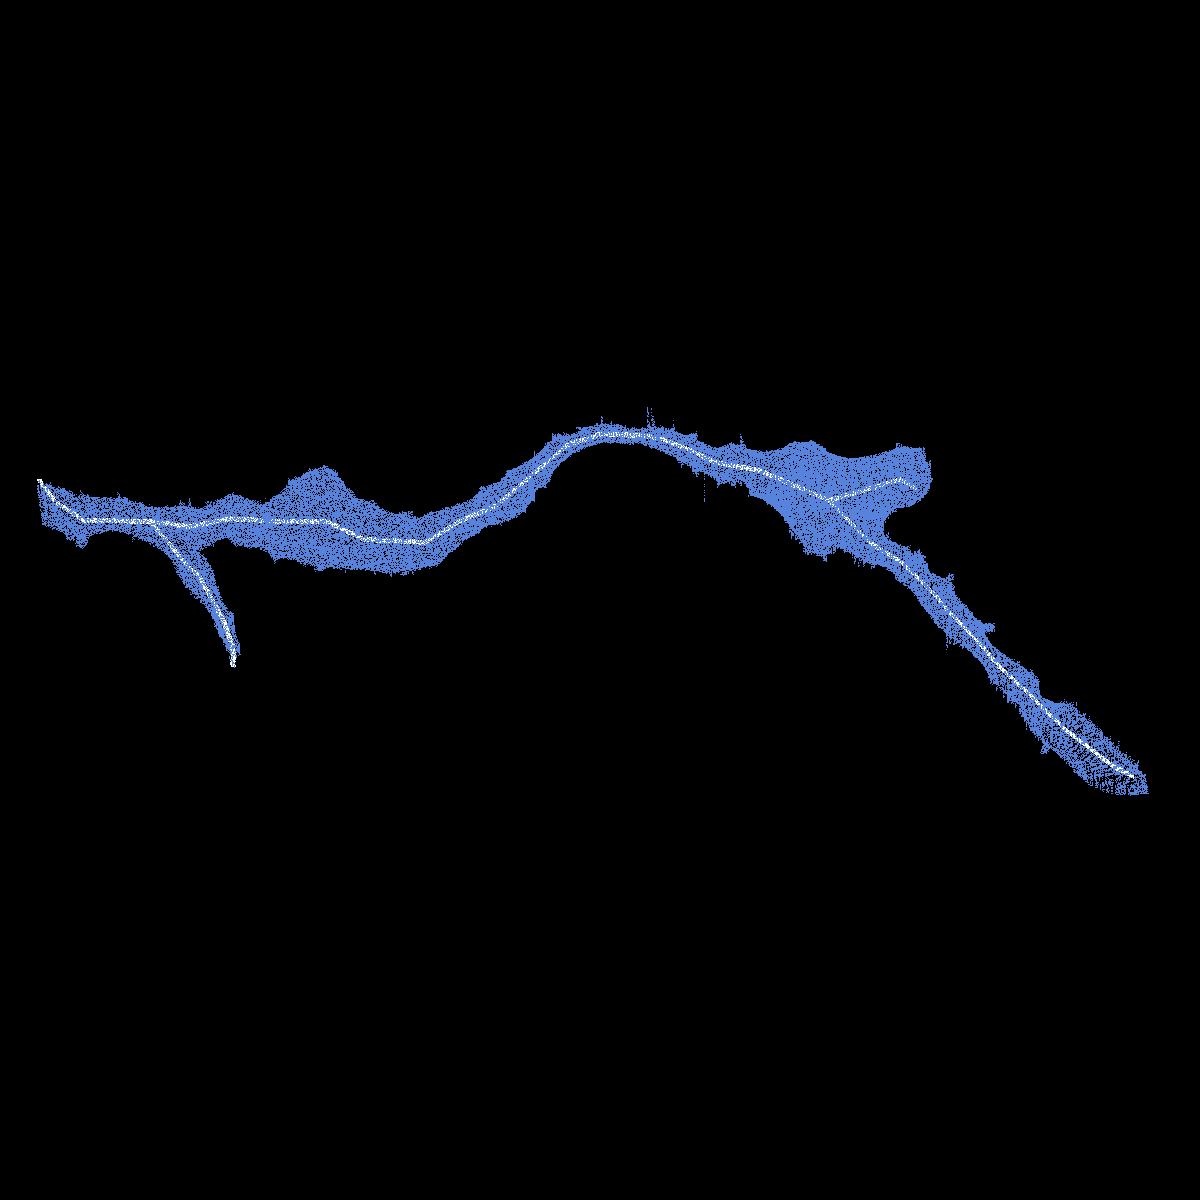
\includegraphics[width=0.92\linewidth]{./figures/skeleton1.png}
	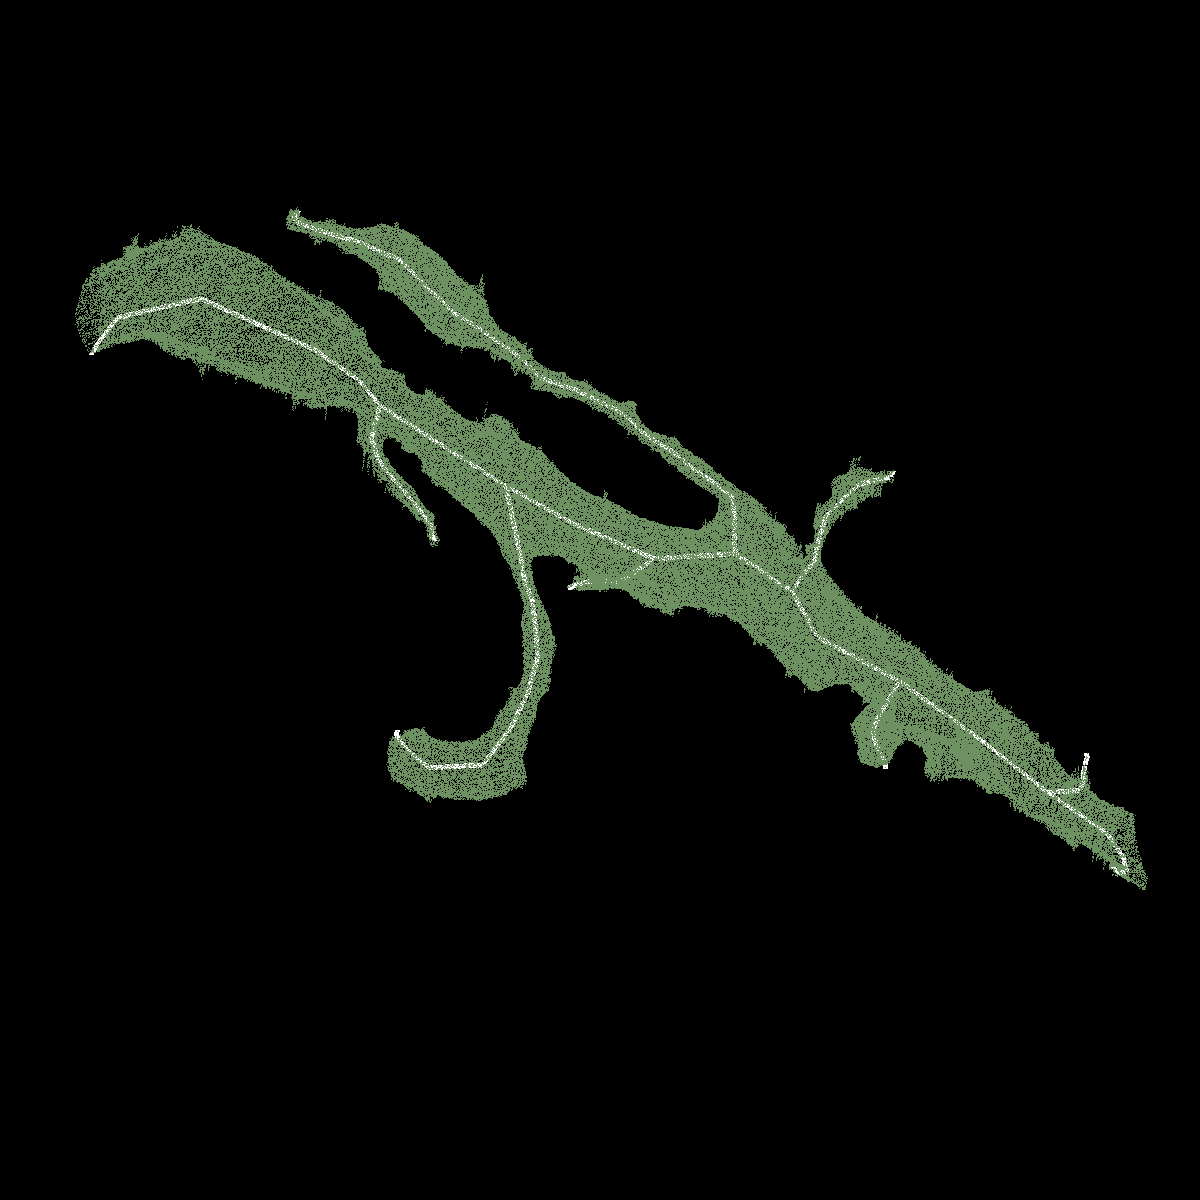
\includegraphics[width=0.92\linewidth]{./figures/skeleton2.png}
	\caption{Skeletons using the TEASER algorithm.}
	\label{fig:skeletonization}
\end{figure}

There are two types of possible errors in image segmentation problems.
A \textit{split error} occurs when there are two segments which should be one. 
A \textit{merge error} happens when one segment should not have been merged. 
Generally, it is much more difficult to correct merge errors than to correct split errors. 
Therefore, we take an oversegmentation of the $EM$ image volume as input so that most of the errors are split errors. 
We identify these split error locations and merge the offending segments.
Section~\ref{sec:neuroproof} discusses two pipelines for generating the oversegmentations. 

From the input segmentation we generate a graph $G$ with nodes $N$ and edges $E$ with weights $w_e$. 
The nodes correspond to unique labels from the segmentation.
There is an edge between all nodes which we consider for merging. 
Ideally, our graph has edges corresponding to all of the segments which were erroneously split with few edges between correctly split segments.
We consider an object's skeleton as a simplified representation of its shape.
We use these skeletons to identify merge candidates and add an edge to the graph.
A CNN produces a probability that two candidates should merge, and we assign the corresponding edge this probability as a weight. 
A multicut heuristic partitions the graph to produce an output segmentation.
Thus there are three major components to our framework: skeletonization for constructing a graph, network training for determining edge weights, and graph-partitioning using a multicut heuristic.

\subsection{Graph Creation}
\label{sec:skeletonization}
\subsubsection{Node Generation}

The simplest node generation strategy creates one node for every unique segment label in the input volume.
However, some of the millions of labels correspond to very small volumes. 
Usually these locations have noisy image data so the pixel-based methods cannot provide enough information to generate a larger segment.
It is difficult to extract useful shape features from these segments because of their small, and often random, appearance. 
We prune these nodes from the graph by removing all segments with fewer than $20,000$ voxels. 
This removes XX\% of segments on a typical connectomics dataset. 

\subsubsection{Edge Generation}

A na\"ive approach to generating edges produces an edge between all adjacent segments.
Two segments $l_1$ and $l_2$ are considered adjacent if there is a pair of adjacent voxels where one has label $l_1$ and the other has label $l_2$. 
NeuroProof and GALA consider all pairs of adjacent segments for merging. 
For us, this method produces too many edges in the graph. 
Therefore we present the following algorithm to identify pairs of segments to consider for merging. 

First, we extract a skeleton from each segment using the TEASER algorithm~\cite{sato2000teasar,zhao2014automatic}.
Figure~\ref{fig:skeletonization} shows the skeletons in white of two segments from the label volume.
These skeletons consist of a sequence of \textit{joints}, locations that are a local maximum distance from the segment boundary, with line segments connecting successive joints. 
We prune the joints that are within $50$ voxels of each other to reduce unnecessary branching.
For the purposes of our algorithm, joints that have only one connected neighbor are referred to as \textit{endpoints}. 
Many of the segments that are erroneously split follow a similar pattern (Figure~\ref{fig:merge_candidates}). 
In these split instances the two skeletons have nearby endpoints.

We identify segments for merge consideration with the following two-pass heuristic.
In the first pass, we iterate over all endpoints $e$ belonging to a segment $S$ and create a set of segments $\mathbb{S}_e^\prime$ that includes all labels that have a single voxel within $t_{low}$ voxels from $e$. 
Oftentimes this first pass produces too many candidates.
In the second pass, we consider all of the segments $\mathbb{S}_e^\prime$ for every endpoint $e$. 
If a segment $S^\prime \in \mathbb{S}_e^\prime$ has an endpoint within $t_{high}$ voxels of $e$, the segment $S$ and $S^\prime$ are considered for merging. 
We store the midpoint between the two endpoints as the ``center" of the potential merge.

\begin{figure}[t]
	\centering
	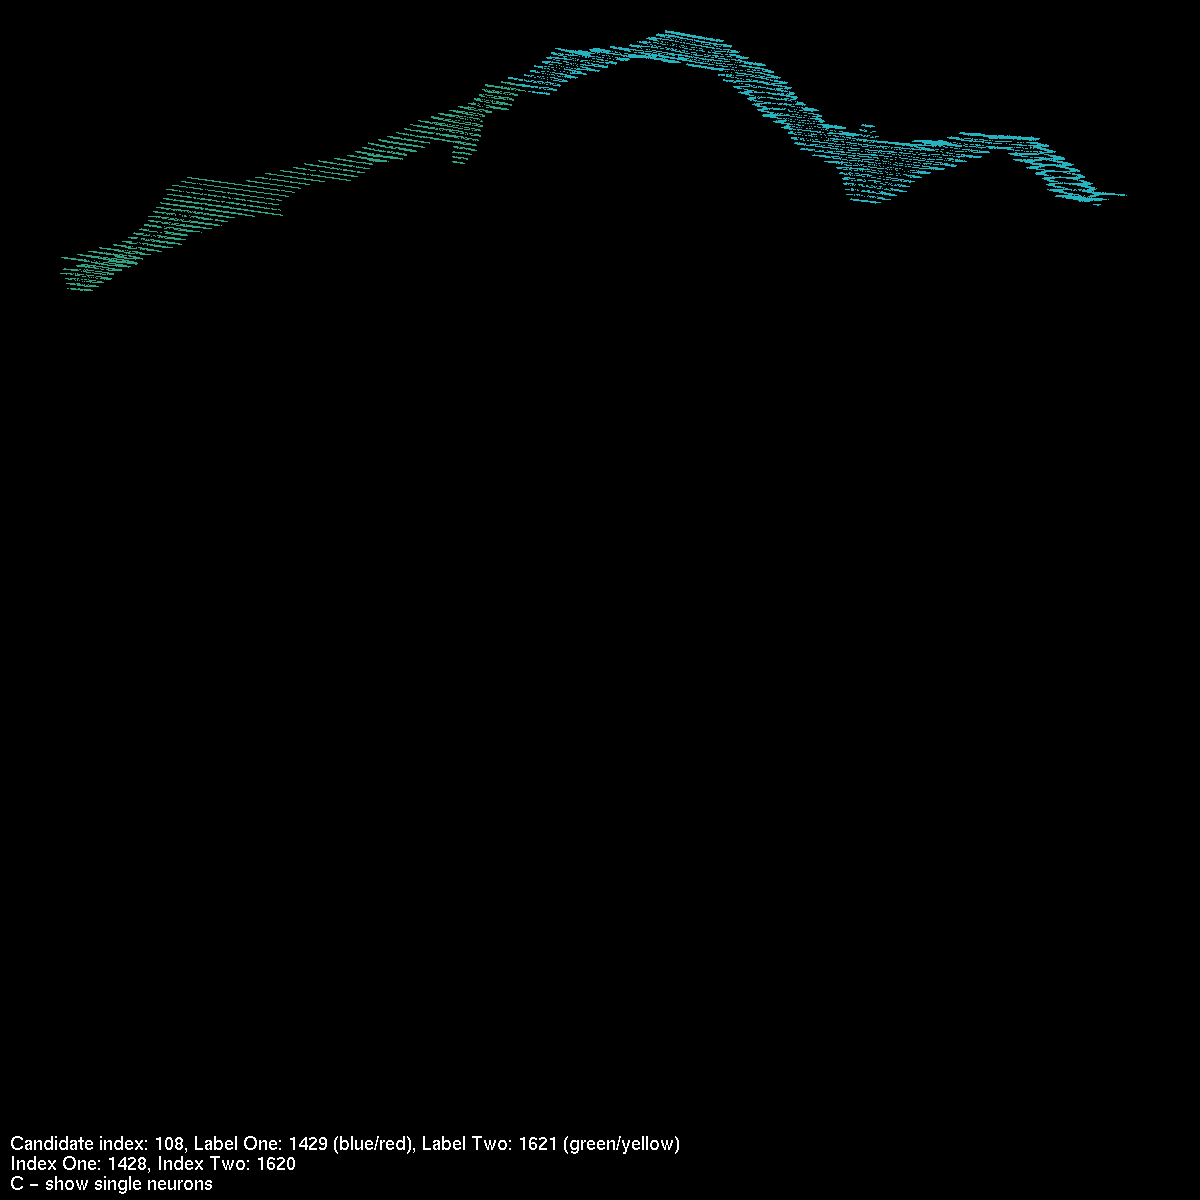
\includegraphics[width=0.92\linewidth]{./figures/split_error1.png}
	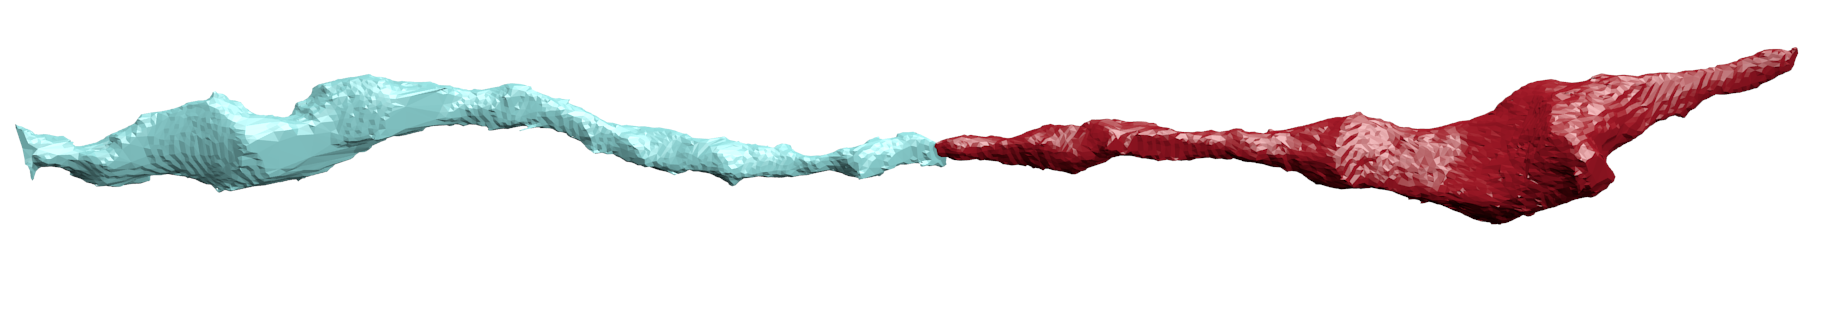
\includegraphics[width=0.92\linewidth]{./figures/split_error2.png}
	\caption{Two erroneously split segments.}
	\label{fig:merge_candidates}
\end{figure}


\subsection{Edge Weights}

Our graph generation algorithm produces 3-D locations that require further consideration for merging. 
To determine which of these segments should actually merge, we train a 3-D CNN using the oversegmentation and the corresponding manually labeled ground truth data (Section~\ref{sec:dataset}).
We extract a cubic region of interest around these locations as input to the CNN. 
These regions of interest provide the local information for the neural network to predict which neighboring segments belong to the same neuron. 

The networks receives three input channels for every voxel in the region of interest around segments $l_1$ and $l_2$. 
The input to all of the channels is in the set $\{-0.5, 0.5\}$. 
The first channel is $0.5$ only if the corresponding voxel has label $l_1$. 
The second channel is $0.5$ only if the corresponding voxel has label $l_2$. 
The third channel is $0.5$ if the corresponding voxel is either $l_1$ or $l_2$. 

Figure~\ref{fig:architecture} provides an overview of our architecture. 
The network architecture has three layers of double convolutions followed by a max pooling step based on the work of Chatfield et al. that found this technique improves on single convolution layers~\cite{chatfield2014return}. 
The first max pooling layer is anisotropic with pooling only in the $x$ and $y$ dimensions.
The filters after the final pooling step are flattened into a 1-D vector which is input into two fully connected layers.
The final layer produces a probability with a sigmoid activation function~\cite{funahashi1989approximate}. 
All of the other activation functions are LeakyReLU~\cite{maas2013rectifier}. 
We use the stochastic gradient descent optimizer with Nesterov's accelerated gradient~\cite{nesterov1983method}. 
There are dropouts of $0.2$ after every pooling layer and the first dense layer, and a dropout of $0.5$ after the final dense layer to prevent overfitting. 
We discuss all other network parameters in Section~\ref{sec:network-parameters}.

\begin{figure*}[t]
	\centering
	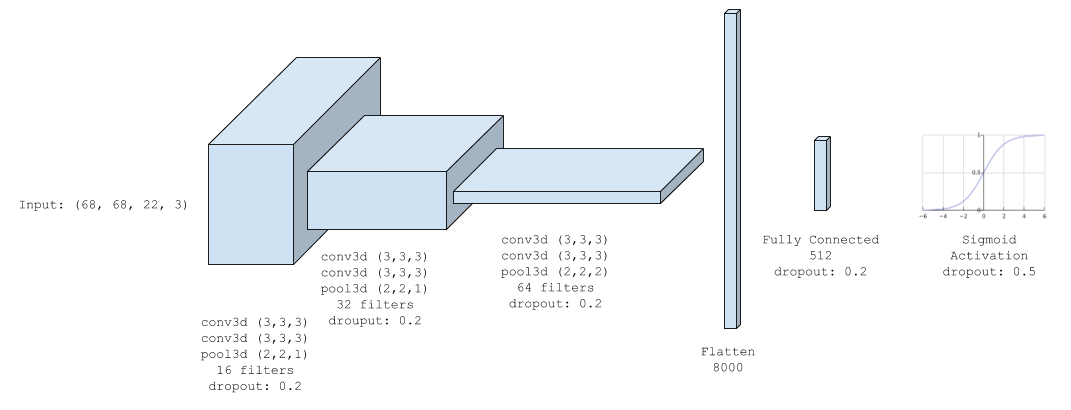
\includegraphics[width=0.95\linewidth]{figures/architecture.png}
	\caption{The architecture for the neural networks follows the \textit{VGG} style of double convolutions followed by a max pooling operation. The number of filters doubles each layer leading to a fully connected layer and a sigmoid activation function.}
	\label{fig:architecture}
\end{figure*}

\subsection{Graph Partitioning}

After constructing the graph structure we apply a graph-based segmentation strategy. 
There are many graph partitioning minimization functions that provide different constraints on their output. 
Neurons in the brain should be acyclic (i.e. the output shape should have a genus of zero). 
We enforce this constraint by finding a multicut partition of the graph that generates a \textit{forest} on the nodes. 
A forest is a partitioning of a graph into a set of trees (i.e. no segment has a cycle). 
There are several heuristics that solve the multicut problem (which is NP-Hard). 
We use the greedy-additive algorithm~\cite{keuper2015efficient}.